\documentclass{article}

\usepackage{tikz}
\usepackage{pgfplots}
\pgfplotsset{compat=newest}
\usepgfplotslibrary{patchplots}


\usetikzlibrary{calc}


%Esperimenti
\usepgfplotslibrary{groupplots}
\usetikzlibrary{arrows} 
	%\usepackage{pgffor}
	
\pagestyle{empty}


%Common symbols
%Common math symbols
	%Number fields
		\newcommand{\Real}{\mathbb{R}}
		\newcommand{\Natural}{\mathbb{N}}
		\newcommand{\Relative}{\mathbb{Z}}
		\newcommand{\Rational}{\mathbb{Q}}
		\newcommand{\Complex}{\mathbb{C}}
	
%equality lingo
	%must be equal
		\newcommand{\mbeq}{\overset{!}{=}} 

% function
	%Domain
		\newcommand{\dom}{\mathrm{dom}}
	%Range
		\newcommand{\ran}{\mathrm{ran}}
	

% Set Theory
	% Power set (insieme delle parti
		\newcommand{\PowerSet}{\mathcal{P}}

%Differential Geometry
	% Atlas
		\newcommand{\Atlas}{\mathcal{A}}
	%support
		\newcommand{\supp}{\textrm{supp}}

	
	
%Category Theory
	%Mor set http://ncatlab.org/nlab/show/morphism
%		\newcommand{\hom}{\textrm{hom}}

%Geometric Lagrangian Mechanics
	% Kinematic Configurations
		\newcommand{\Conf}{\mathtt{C}}
	%Solutions Space
		\newcommand{\Sol}{\mathtt{Sol}}
	%Lagrangian class
		\newcommand{\Lag}{\mathsf{Lag}}
	%Lagrangiana
		\newcommand{\Lagrangian}{\mathcal{L}}
	%Data
		\newcommand{\Data}{\mathsf{Data}}
	%unique solution map
		\newcommand{\SolMap}{\mathbf{s}}
	%Classical Observables
		\newcommand{\Obs}{\mathcal{E}}	
	%Phase Space
		\newcommand{\Phase}{\mathcal{M}}	

		\
		
%Peierls (per non sbagliare più)
		\newcommand{\Pei}{Peierls}


%Funzione 3D
\pgfmathdeclarefunction{F}{2}{\pgfmathparse{5*(2+(sin((#2-1.7)*80)*(#2/6)^3)+0.1*cos(#1*80)*(2^(-#2^2)))}}
%{\pgfmathparse{3000-1000*sin(#1)+1500*(#2/6)^5}}
%*(#2/6)^3

\begin{document}
%\/\/\/\/\/\/\/\/\/\/\/\/\/\/\/\/\/\/\/\/\/\/\/\/\/\/\/\/\/\/\/\/\/\/\/\/\/\/\/\/\/\/\/\/\/\/\/\/\/\/\/\/\/\/\/\/\/\/\/\/\/\/\/\/\/\/
\section{Figura 0}
La rappresentazione 2D dello spazio delle configurazioni Cinematiche\\
\begin{tikzpicture}
\begin{axis}[axis lines=none,clip=false]

	% Il riquadro di \Conf
	\addplot[color=black] coordinates {
		(8,6) (0,6) (0,0)(8,0)(8,6)
		}node [pos=1,pin={0:$\Conf$},inner sep=0pt] {};

	% la retta di \Sol
	\addplot[color=red] coordinates {
		(0,2)
		(8,2)
	}node [pos=1,pin={0:$\Sol$},inner sep=0pt] {};
	
	% Zero section
	\node[label={270:{$0$}},circle,fill,inner sep=1pt] at (axis cs:1.25,2) {};
	% Fixed Solution
	\node[label={270:{$\phi_0$}},circle,fill,inner sep=1pt] at (axis cs:5,2) {};

	% La curva di \Sol_\epsilon
	\addplot[color=gray,smooth] coordinates {
	(6,6) (3.5,4.5)(6,3)
	(5,2) (6,1)
	(3.5,0) 
	}node [pos=1,pin={270:$\phi_\epsilon$},inner sep=0pt] {};


\end{axis}
\end{tikzpicture}



%\/\/\/\/\/\/\/\/\/\/\/\/\/\/\/\/\/\/\/\/\/\/\/\/\/\/\/\/\/\/\/\/\/\/\/\/\/\/\/\/\/\/\/\/\/\/\/\/\/\/\/\/\/\/\/\/\/\/\/\/\/\/\/\/\/\/
\section{Figura 1}
 Le variazioni di Peierels\\
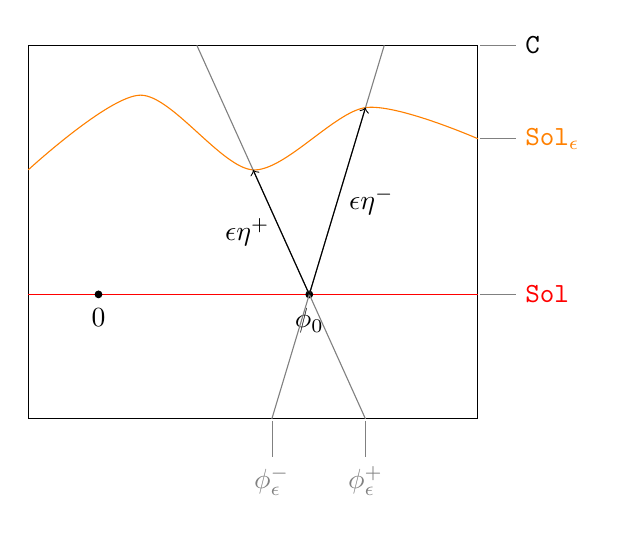
\begin{tikzpicture}
\begin{axis}[axis lines=none,clip=false]

	% Il riquadro di \Conf
	\addplot[color=black] coordinates {
		(8,6) (0,6) (0,0)(8,0)(8,6)
		}node [pos=1,pin={0:$\Conf$},inner sep=0pt] {};

	% la retta di \Sol
	\addplot[color=red] coordinates {
		(0,2)
		(8,2)
	}node [pos=1,pin={0:$\Sol$},inner sep=0pt] {};
	
	% Zero section
	\node[label={270:{$0$}},circle,fill,inner sep=1pt] at (axis cs:1.25,2) {};
	% Fixed Solution
	\node[label={270:{$\phi_0$}},circle,fill,inner sep=1pt] at (axis cs:5,2) {};

	% La curva di \Sol_\epsilon
	\addplot[color=orange,smooth] coordinates {
	(0,4) (2,5.2)(4,4)(6,5)(8,4.5)
	}node [pos=1,pin={0:$\Sol_\epsilon$},inner sep=0pt] {};

	%Variation
	\addplot[color=gray] coordinates {
		(3,6)
		(6,0)
	}node [pos=1,pin={270:$\phi_\epsilon^+$},inner sep=0pt] {};
	\addplot[color=gray] coordinates {
		(6.33333,6)
		(4.33333,0)
	}node [pos=1,pin={270:$\phi_\epsilon^-$},inner sep=0pt] {};
	
	%Perturbation
	\addplot[->] coordinates
           {(5,2) (4,4)}node [pos=0.5,label={180:$\epsilon \eta^+$},inner sep=0pt] {};
	\addplot[->] coordinates
           {(5,2) (6,5)}node [pos=0.5,label={0:$\epsilon \eta^-$},inner sep=0pt] {};


\end{axis}
\end{tikzpicture}


%\/\/\/\/\/\/\/\/\/\/\/\/\/\/\/\/\/\/\/\/\/\/\/\/\/\/\/\/\/\/\/\/\/\/\/\/\/\/\/\/\/\/\/\/\/\/\/\/\/\/\/\/\/\/\/\/\/\/\/\/\/\/\/\/\/\/
\section{Figura 2}
Rappresentazione di funzionali e di effetto\\
\begin{tikzpicture}
\begin{axis}[axis lines=none,clip=false,view={30}{30},]

	%Funzionale sulle configurazioni
	\addplot3[    surf,    colormap/greenyellow,% mesh, color=gray
	,domain=0:8,y domain=0:6]
	{F(x,y)};

	% Il riquadro di \Conf
	\addplot3[color=black] coordinates {
		(8,6,0) (0,6,0) (0,0,0)(8,0,0)(8,6,0)
		}node [pos=1,pin={270:$\Conf$},inner sep=0pt] {};

	%Valore B(\phi_0)$
	\node[label={135:{\tiny $B(\phi_0)$}},circle,fill,inner sep=1pt] at (axis cs:5,2,{F(5,2)}) {};
	

	% Curve parametrizzate sulla superficie (le spezzo a metà così riesco a mettere bene il vettore tangente
		\addplot3[red,domain=0:2/3,variable=\t,samples y=0] ({3+3*t},{6-6*t},{F(3+3*t,6-6*t)})
			node [pos=0,pin={30:{\tiny $ B(\phi_\epsilon^+)$}},inner sep=0pt] {}
       		node[pos=1,sloped,inner sep=0cm,above,
  	    				anchor=south west,
   	  	 				minimum height=(10+50)*0.03cm,minimum width=(10+50)*0.03cm]
    	  				(P 0) {}		%nodo di phi_0
			;
		 \draw[-latex,color=black] (P 0.south west) -- (P 0.south east)node [pos=0.85,label={90:{\tiny $ \EffectOp_\chi^+ B ( \phi_0)$}}] {};
		 \addplot3[red,domain=2/3:1,variable=\t,samples y=0] ({3+3*t},{6-6*t},{F(3+3*t,6-6*t)});

		\addplot3[red,domain=0:(2/3),variable=\t,samples y=0] ({6.33333-2*t},{6-6*t},{F(6.33333-2*t,6-6*t)})
			node [pos=0,pin={30:{\tiny $ B(\phi_\epsilon^-)$}},inner sep=0pt] {}
       		node[pos=1,sloped,inner sep=0cm,above,
  	    				anchor=south west,
   	  	 				minimum height=(10+50)*0.03cm,minimum width=(10+50)*0.03cm]
    	  				(P 1) {}		%nodo di phi_0
			;
		 \draw[-latex,color=black] (P 1.south west) -- (P 1.south east) node [pos=0.75,label={45:{\tiny $ \EffectOp_\chi^- B ( \phi_0)$}}] {}; 
		 \addplot3[red,domain=(2/3):1,variable=\t,samples y=0] ({6.33333-2*t},{6-6*t},{F(6.33333-2*t,6-6*t)});



	%\\\\\\\\\\\\\\Parte 2d)\\\\\\\\\\\\\\
	% la retta di \Sol
	\addplot[color=red] coordinates {
		(0,2)
		(8,2)
	}node [pos=1,pin={270:$\Sol$},inner sep=0pt] {};
	
	% Zero section
	\node[label={270:{$0$}},circle,fill,inner sep=1pt] at (axis cs:1.25,2) {};
	
	% Fixed Solution
	\node[label={270:{$\phi_0$}},circle,fill,inner sep=1pt] at (axis cs:5,2) {};

	% La curva di \Sol_\epsilon
	\addplot[color=orange,smooth] coordinates {
	(0,4) (2,5.2)(4,4)(6,5)(8,4.5)
	}node [pos=1,pin={270:$\Sol_\epsilon$},inner sep=0pt] {};

	%Variation
	\addplot[color=gray] coordinates {
		(3,6)
		(6,0)
	}node [pos=1,pin={270:$\phi_\epsilon^+$},inner sep=0pt] {};
	\addplot[color=gray] coordinates {
		(6.33333,6)
		(4.33333,0)
	}node [pos=1,pin={270:$\phi_\epsilon^-$},inner sep=0pt] {};
	
	%Perturbation
	\addplot[->] coordinates
           {(5,2) (4,4)}node [pos=0.5,label={180:$\epsilon \eta^+$},inner sep=0pt] {};
	\addplot[->] coordinates
           {(5,2) (6,5)}node [pos=0.5,label={0:$\epsilon \eta^-$},inner sep=0pt] {};


\end{axis}
\end{tikzpicture}



%\/\/\/\/\/\/\/\/\/\/\/\/\/\/\/\/\/\/\/\/\/\/\/\/\/\/\/\/\/\/\/\/\/\/\/\/\/\/\/\/\/\/\/\/\/\/\/\/\/\/\/\/\/\/\/\/\/\/\/\/\/\/\/\/\/\/
\section{Figura 3}
 Il Caso dei funzionali lagrangiani semplici\\
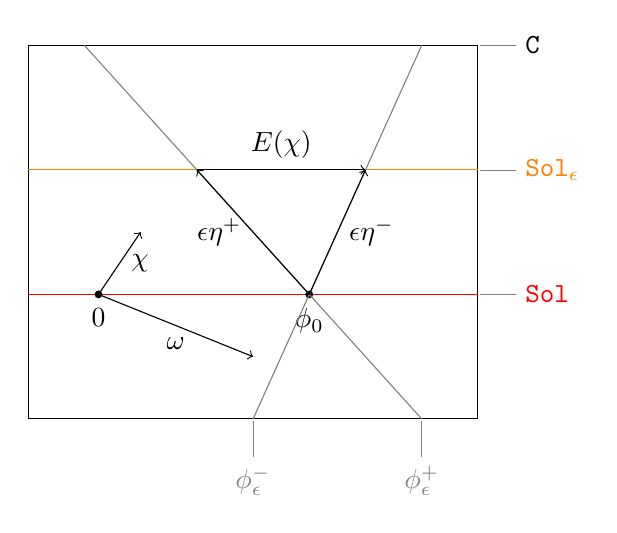
\begin{tikzpicture}
\begin{axis}[axis lines=none,clip=false]

	% Il riquadro di \Conf
	\addplot[color=black] coordinates {
		(8,6) (0,6) (0,0)(8,0)(8,6)
		}node [pos=1,pin={0:$\Conf$},inner sep=0pt] {};

	% la retta di \Sol
	\addplot[color=red] coordinates {
		(0,2)
		(8,2)
	}node [pos=1,pin={0:$\Sol$},inner sep=0pt] {};
	
	% Zero section
	\node[label={270:{$0$}},circle,fill,inner sep=1pt] at (axis cs:1.25,2) {};
	% Fixed Solution
	\node[label={270:{$\phi_0$}},circle,fill,inner sep=1pt] at (axis cs:5,2) {};

	% La curva di \Sol_\epsilon
	\addplot[color=orange] coordinates {
	(0,4)(8,4)
	}node [pos=1,pin={0:$\Sol_\epsilon$},inner sep=0pt] {};

	%Variation
	\addplot[color=gray] coordinates {
		(1,6)
		(7,0)
	}node [pos=1,pin={270:$\phi_\epsilon^+$},inner sep=0pt] {};
	\addplot[color=gray] coordinates {
		(7,6)
		(4,0)
	}node [pos=1,pin={270:$\phi_\epsilon^-$},inner sep=0pt] {};
	
	%Perturbation
	\addplot[->] coordinates
           {(5,2) (3,4)}node [pos=0.5,label={180:$\epsilon \eta^+$},inner sep=0pt] {};
	\addplot[->] coordinates
           {(5,2) (6,4)}node [pos=0.5,label={0:$\epsilon \eta^-$},inner sep=0pt] {};

	%AdvancedMinusRetarded
	\addplot[->] coordinates
           {(3,4) (6,4)}node [pos=0.5,label={90:$E (\chi)$},inner sep=0pt] {};
           
	%LagrangianDensities
	\addplot[->] coordinates
           {(1.25,2) (4,1)}node [pos=0.5,label={270:$\omega$},inner sep=0pt] {};	
	\addplot[->] coordinates
           {(1.25,2) (2,3)}node [pos=0.5,label={0:$\chi$},inner sep=0pt] {};		
	
	

\end{axis}
\end{tikzpicture}


%\/\/\/\/\/\/\/\/\/\/\/\/\/\/\/\/\/\/\/\/\/\/\/\/\/\/\/\/\/\/\/\/\/\/\/\/\/\/\/\/\/\/\/\/\/\/\/\/\/\/\/\/\/\/\/\/\/\/\/\/\/\/\/\/\/\/
\section{Figura 4}
Immagine della variazione geodetica in un piano 2d

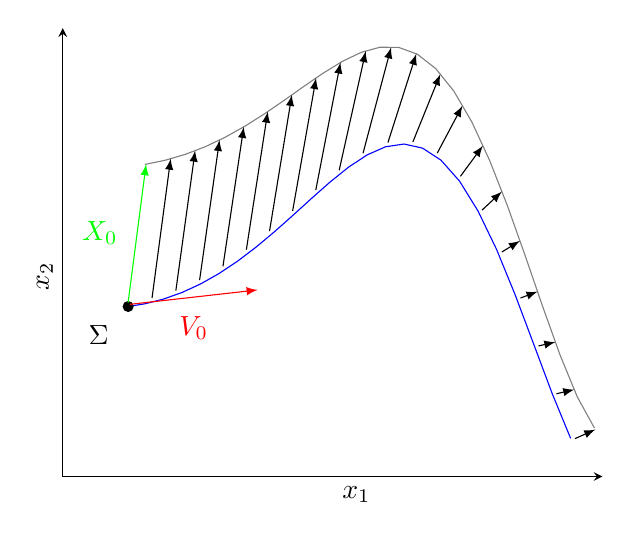
\begin{tikzpicture}
\begin{axis}[	axis x line=bottom, axis y line=left,
						ticks=none,
						xlabel={$x_1$},ylabel={$x_2$},
						xlabel style={below right},ylabel style={above left},
						xmin=-1, xmax=16, ymin=-1.8, ymax=3
						]
 
 		% Geodesica di partenza
		\addplot[blue,domain=1:15,variable=\t] ({t},{sin(x^2)*x^(1/4)})		
		  \foreach \p in {0,1,...,20}{						%punti per ottenere il vettore variazione
      		node[sloped,inner sep=0cm,above,pos=\p/20,
      			anchor=south west]
      			(N \p){}
  			};	

		% Geodesica Variata
		\addplot[gray,domain=1:15,variable=\t] ({t+0.5*(1+sin(t*10))},{sin(x^2)*x^(1/4)+(1 +0.5*cos(t*10))})
			 \foreach \p in {0,1,...,20}{						%punti per ottenere il vettore variazione
    	  		node[	sloped,inner sep=0cm,above,pos=\p/20,
      						anchor=south west]
      				(M \p){}
  			};	

		%I Dati Iniziali
		\fill (N 0.south) circle [radius=2pt]node [label={225:{$\Sigma$}}]  {};  

		\draw[-latex,color=green] (N 0) -- (M 0) node [pos=0.5,label={180:{$X_0$}}]  {};    

		%La velocità iniziale la metto a mano in modo che si legga chiaramente 
		\draw[-latex,color=red] (N 0) -- ($(N 0) + (-28:3.5)$) node [pos=0.5,label={270:{$V_0$}}]  {};
		

\end{axis}

	%Lo Jacobi Field
    \foreach \p in {1,2,...,20} {
      \draw[-latex,color=black] (N \p) -- (M \p);
    }

    

\end{tikzpicture}

\section{Figura 5}
Initial data set

\begin{tikzpicture}
\begin{axis}[,clip=false,
						axis x line=bottom, axis y line=left,
						ticks=none,
						xmin=-1, xmax=16, ymin=-1, ymax=9
						]
	
	%Riquadro che simboleggia Data
	\addplot[dashed,color=gray] coordinates {
		(1,1) (14,1) (14,7)(1,7)(1,1)
		}node [pos=1,pin={270:$\Data$},inner sep=0pt] {};


	%Il piano R2 del vettore iniziale
		\draw[->,color=black] (2,3) -- (6,3);
		\draw[->,color=black] (3,2) -- (3,6);

	%Il piano R2 della velocità iniziale 
		\draw[->,color=black] (9,3) -- (13,3);
		\draw[->,color=black] (10,2) -- (10,6);

	%è un prodotto cartesiano
		\node[] at (7.5,4.5) {$\times$};

	%I dati iniziali
		\draw[-latex,color=green] (3,3) -- (4,6) node [pos=0.5,label={180:{$X_0$}}]  {};    
		\draw[-latex,color=red] (10,3) -- (12.5,3.7) node [pos=0.5,label={270:{$V_0$}}]  {};

\end{axis}

\end{tikzpicture}

\section{Figura 6}
Unire le due precedenti
\begin{tikzpicture}
\begin{axis}[,clip=false,
						axis x line=bottom, axis y line=left,
						ticks=none,
						xmin=-1, xmax=16, ymin=-1, ymax=9
						]
	
	%Riquadro che simboleggia Data
	\addplot[dashed,color=gray] coordinates {
		(1,1) (14,1) (14,7)(1,7)(1,1)
		}node [pos=1,pin={270:$\Data$},inner sep=0pt] {};
\end{axis}

\begin{axis}[,clip=false,
						axis x line=bottom, axis y line=left,
						ticks=none,
						xmin=-1, xmax=16, ymin=-1, ymax=9
						]
	
	%Riquadro che simboleggia Data
	\addplot[dashed,color=red] coordinates {
		(1,3) (2,1) (5,-1)(1,7)(1,1)
		}node [pos=1,pin={270:$\Data$},inner sep=0pt] {};
\end{axis}

\end{tikzpicture}



%\/\/\/\/\/\/\/\/\/\/\/\/\/\/\/\/\/\/\/\/\/\/\/\/\/\/\/\/\/\/\/\/\/\/\/\/\/\/\/\/\/\/\/\/\/\/\/\/\/\/\/\/\/\/\/\/\/\/\/\/\/\/\/\/\/\/

\section{Esperimenti}
 \begin{tikzpicture}[allow upside down]
\draw[red,line width=1pt] (0,0) .. controls ++(1,6) and ++(-1,2) .. (10,4)
      node[sloped,inner sep=0cm,above,pos=.5,
      anchor=south west,
      minimum height=(10.5)*0.3cm,minimum width=(10.5)*.3cm](N){};

\path (N.south west)%
           edge[-stealth',blue] node[left] {$\vec{ n}$} (N.north west)
           edge[-stealth',blue] node[above] {$\vec{ t}$} (N.south east);
\draw[-stealth',gray]  (N.south west)  --%
      node[below] {$\vec{t_a}$} (N.south west -| N.south east); 
\draw[-stealth',gray]  (N.south west)  --%
      node[right] {$\vec{t_o}$} (N.south west |- N.south east);

  \end{tikzpicture}  
  
  
 \subsection{Vettore tangente}
 \begin{tikzpicture}[allow upside down,x=1.5cm,y=1.4cm]
    \draw[red,thick] (0,0)
    .. controls +(right:1cm) and +(left:2cm) .. (2,2)
        node[sloped,inner sep=0cm,above,pos=50*0.01,
  	    anchor=south west,
   	  	 minimum height=(10+50)*0.03cm,minimum width=(10+50)*0.03cm]
    	  (N 50){}
    ;
      \draw[-latex,color=black] (N 50.south west) -- (N 50.south east);
  \end{tikzpicture}

\subsection{Vettore Tangente con FOREACH}
%\url{http://tex.stackexchange.com/questions/219747/normalized-tangent-vectors-along-a-curve}
 \begin{tikzpicture}[allow upside down,x=1.5cm,y=1.4cm]
    \draw[red,thick] (0,0)
    .. controls +(right:6cm) and +(left:4cm) .. (2,6)
        \foreach \p in {0,10,...,100} {
      node[sloped,inner sep=0cm,above,pos=\p*0.01,
      anchor=south west,
      minimum height=(10+\p)*0.03cm,minimum width=(10+\p)*0.03cm]
      (N \p){}
    }
    ;
    \foreach \p in {0,10,...,100} {
      \draw[-latex,color=black] (N \p.south west) -- (N \p.south east);
    }
  \end{tikzpicture}
  
  
  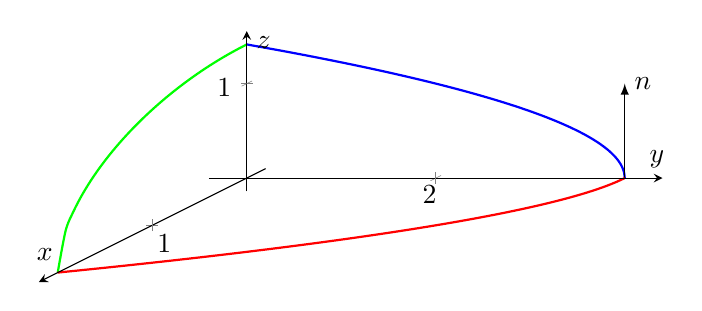
\begin{tikzpicture}
\begin{axis}[
    scale=2,
    x={(-0.6cm,-0.3cm)}, y={(.6cm,0.0cm)}, z={(0cm,.6cm)},
    xlabel={$x$}, ylabel={$y$}, zlabel={$z$},
    axis lines=middle, axis on top,
    xtick={1}, ytick={2},ztick={1},
    enlargelimits=true
    ]

\addplot3[
    samples y=0,
    smooth, thick, color=blue,
    domain=0:sqrt(2)
    ] ({0},{4-2*x^2},{x});
\draw [-latex] (current plot begin) -- +(axis direction cs:0,0,1) node [anchor=west] {$n$};

\addplot3[
    samples y=0,
    smooth, thick, color=green,
    domain=0:2
    ] ({x},{0},{sqrt(2-x^2/2)});
\addplot3[
    samples y=0,
    smooth, thick, color=red,
    domain=0:2
    ] ({x},{4-x^2},{0});

\end{axis}
\end{tikzpicture}

\subsection{Separazione Tra due cammini}
% \url{http://tex.stackexchange.com/questions/230729/how-to-draw-inward-arrows-between-two-paths}


\subsection{Figure diverse collegate da freccia}
%http://tex.stackexchange.com/questions/58360/how-to-draw-a-joining-line-between-two-picture-tikz-pgf
    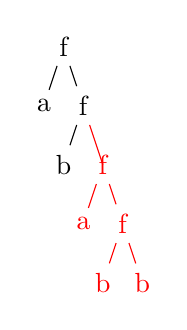
\begin{tikzpicture}[remember picture,scale=0.5] 
    \tikzstyle{level 1}=[sibling distance=10mm] 
    \node{f} 
    child{node{a}}
    child{node{f} child{node{b}} child{[red] node (f1) {f }   child{node{a}} child{node{f} child{node{b}}child{node{b}}}      }}
    ;
    \end{tikzpicture}
   \begin{tikzpicture}[remember picture,scale=0.5] 
   \tikzstyle{level 1}=[sibling distance=10mm] 
   \node (f2) {f} 
    child{node{a}}
    child{node{f} child{node{b}} child{ node{f }   child{node{a}} child{node{g} child[missing] child{node{a}}}      }}
    ;
\draw (f1) .. controls (-3,3) .. (f2);
   \end{tikzpicture}

\subsection{Test ForEach}
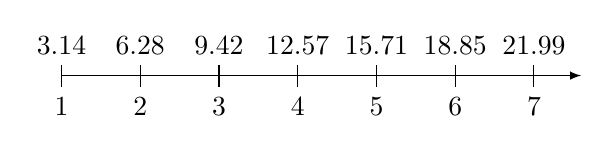
\begin{tikzpicture}

\foreach \x in {1,...,7} {
    \pgfmathsetmacro\result{\x * pi}
    \draw (\x,-4pt) -- (\x,4pt)
        node [below,yshift=-2ex] {\x}
        node [above] {\pgfmathprintnumber{\result}};
}

\draw [-latex] (1,0) -- (7.6,0);

\end{tikzpicture}

\subsection{Patatoidi}
\begin{tikzpicture}
\begin{axis}[axis lines=none,clip=false,
						axis x line=bottom, axis y line=left,
						ticks=none,
						xmin=-1, xmax=16, ymin=-1, ymax=9
						]
	
	\addplot[	patch,mesh,% without mesh, pgfplots tries to fill
						patch type=quadratic spline,color=black]
		coordinates {
		(0,0)  (0,4) (-0.5,2)
		(0,4)  (0,8) (-0.5,6)
		(0,8)(7.5,8)(3.75,8.5)
		(7.5,8)(15,8)(11.25,8.5)
		(15,0)  (15,4) (15.5,2)
		(15,4)  (15,8) (15.5,6)
		(0,0)(7.5,0)(3.75,-0.5)
		(7.5,0)(15,0)(11.25,-0.5)
	};
	\draw (0,0) .. controls (1,1) .. (4,0)
      (5,0) .. controls (6,0) and (6,1) .. (5,2);


\end{axis}

\end{tikzpicture}

\end{document}

